\frontmatter

\pagestyle{empty}
\begin{titlepage}
  
  \begin{center}
  ~ 
  \vspace{30mm} 

  {\huge MODELING THE CRYOSPHERE WITH FEniCS}
  
  \vspace{8mm} 
  
  By
  
  \vspace{8mm}
  
  E.~M.~Cummings

  \vspace{20mm}
  
  \begin{figure}[H]
    \centering
      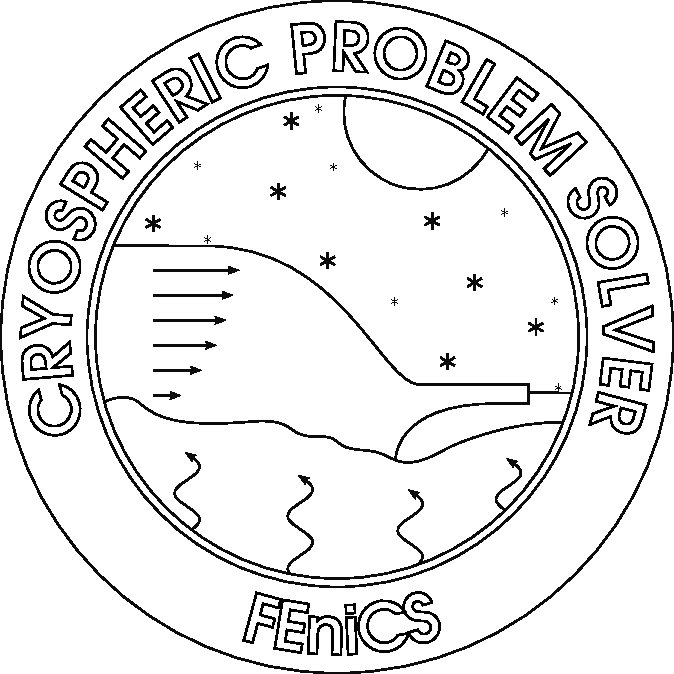
\includegraphics[width=0.6\linewidth]{images/cslvr_mono.pdf}
  \end{figure}
    
  \end{center}

  \newpage
  
  \begin{center}
  
  \
  
  \vspace{8cm}
  
  \copyright\ COPYRIGHT
  
  \vspace{5mm}
  
  by
  
  \vspace{5mm}
  
  Evan Michael Cummings
  
  \vspace{5mm}
  
  \the\year
  
  \vspace{5mm}
  
  All Rights Reserved
  
  \end{center}
  
  \newpage
  
  \begin{table*}[t]
  \centering
  \begin{tabular}{p{50mm}}
    \begin{flushleft}
      To my parents, without whom this project may never have been completed.
    \end{flushleft}
  \end{tabular}
  \end{table*}

\end{titlepage}

\pagestyle{headings}

\tableofcontents
 
\addcontentsline{toc}{chapter}{List of Figures}
\listoffigures
\addcontentsline{toc}{chapter}{List of Tables}
\listoftables
\addcontentsline{toc}{chapter}{List of Algorithms}
\listofalgorithms

\setcounter{tocdepth}{-1}
\addcontentsline{toc}{chapter}{Preface}
\setcounter{tocdepth}{3}
\markboth{}{} % prevent chapter title from last chapter to appear here

\chapter*{Preface}

  This manuscript is a collection of problems and solutions related to modeling the cryosphere using the finite element software FEniCS.  Included is an introduction to the finite element method; solutions to a variety of problems in one, two, and three dimensions; an overview of popular stabilization techniques for numerically-unstable problems; and an introduction to the governing equations of ice-sheet dynamics with associated FEniCS implementations.  The software developed for this project, Cryospheric Problem Solver (\CSLVR), is fully open-source and has been designed with the goal of simplifying many common tasks associated with modeling the cryosphere.  \CSLVR possesses the ability to download popular geological and geographical data, easily convert between geographical projections, develop sophisticated two- or three-dimensional finite-element meshes, convert data between many popular formats, and produce production-quality images of data.  Scripts are presented which model the flow of ice using geometry defined by mathematical functions and observed Antarctic and Greenland ice-sheets data.  A new way of solving the internal energy distribution of ice to match observed intra-ice water contents within temperate regions is thoroughly explained.

The software newly presented in this manuscript, \CSLVR, is largely built from the finite-element software FEniCS \citep{logg_2012}.  \CSLVR solves PDE-constrained-optimization problems through the use of Dolfin-Adjoint \citep{farrell_2013}, which in turn utilizes the IPOPT framework \citep{waechter_2006} compiled with the Harwell Subroutine Library, a collection of Fortran codes for large scale scientific computation (\url{http://www.hsl.rl.ac.uk/}).  All \CSLVR source code is written in the Python programming language (Python Software Foundation, \url{http://www.python.org}).  Countless numerical calculations were accomplished throughout the code-generation process using NumPy and SciPy \citep{annoortvanvanderwalt_2011} via the interactive terminal IPython \citep{perez_2007}.  The meshes used for the Greenland and Antarctic simulations were created with GMSH \citep{geuzaine_2009}.  All of the code-generated figures were created with Matplotlib \citep{hunter_2007}.  All hand-drawn-vector images were created with the open-source-vector-graphics-software Inkscape.  Paraview \citep{ahrens_2005} was used extensively to investigate simulation results and generate figures of three-dimensional data.  Finally, this manuscript was compiled by the invaluable document-creation software \LaTeX.

Special thanks are given to the following people: my thesis committee for taking the time to provide insight and criticism; Robyn Berg for her thoughtful support throughout my undergraduate and graduate career at the University of Montana; all the faculty in the Departments of Computer Science and Mathematics; The University of Montana Group for Quantitative Study of Snow and Ice for providing many thought-provoking discussions and intuition pertaining to the nature of ice-sheets and glaciers; Douglas Brinkerhoff for creating the software VarGlaS \citep{brinkerhoff_2013} from which \CSLVR evolved; and finally Jesse Johnson for his encouragement, support, and guidance.
